
%(BEGIN_QUESTION)
% Copyright 2014, Tony R. Kuphaldt, released under the Creative Commons Attribution License (v 1.0)
% This means you may do almost anything with this work of mine, so long as you give me proper credit

Denne løsemiddeltanken holdes oppvarmet til 95 grader F av en dampvarmeveksler inne i tanken.  Damp slippes inn i varmeveksler-"sløyfen" gjennom temperaturkontrollventil TCV-105, og går ut av sløyfen gjennom en damputlufter:

$$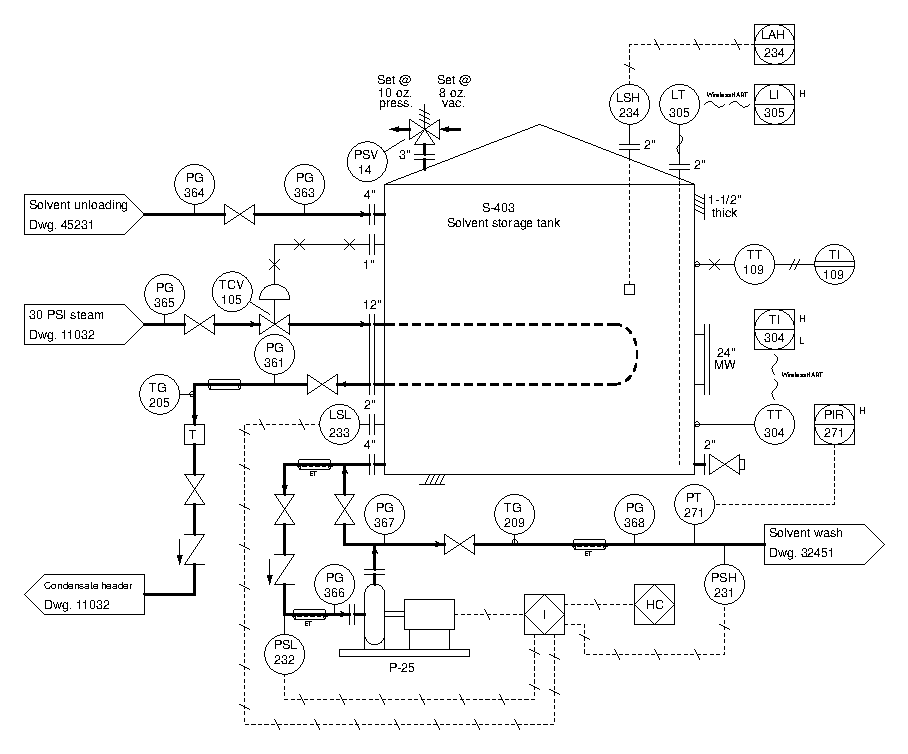
\includegraphics[width=15.5cm]{i0006rx01.eps}$$

Anta at du en dag ser at trykkmåler PG-361 viser 22 PSI mens temperaturmåler TG-205 viser 234 grader F.  Basert på denne informasjonen, avgjør om væsken i røret er {\it damp} (gass) eller {\it vann} (væske).  Forklar hvordan du kom fram til dette.

\vfil 

\underbar{file i00043}
\eject
%(END_QUESTION)





%(BEGIN_ANSWER)

Dette er et vurdert spørsmål -- ingen svar eller hint gis!

%(END_ANSWER)





%(BEGIN_NOTES)

Væsken i dette røret er vann, forutsatt at begge målerne er korrekte.  Ifølge damptabell er metningstemperaturen for vann ved 22 PSIG (36.7 PSIA) omtrent 262 grader F.  Med andre ord må vann ha 262 $^{o}$F for å koke ved et trykk på 22 PSIG.  Siden røret er kaldere enn 262 $^{o}$F, vet vi at røret må inneholde (ikke-kokende) vann og ingen damp.

\vskip 10pt

En annen tilnærming er å slå opp metningstrykket ved den gitte temperaturen 234 grader F.  Her finner vi at trykket er 22.37 PSIA, som er lavere enn 22 PSIG (36.7 PSIA) oppgitt i oppgaven.  Dette betyr at det er tilstrekkelig trykk i systemet til å holde vannet i en ikke-kokende (fullstendig væske) tilstand, og derfor kan det ikke være damp.


%INDEX% Physics, heat and temperature: saturated steam pressure versus temperature
%INDEX% Physics, heat and temperature: steam table
%INDEX% Process: solvent storage tank (realistic P&ID shown)

%(END_NOTES)
